\section{Kotlin/JS}\label{chapter:kotlin_js}

Podczas wyboru języka programowania działającego w AWS Lambda częstym kryterium może być czy język jest kompilowany, czy interpretowany.
Kotlin to domyślnie język kompilowany, jednak poprzez projekt Kotlin Multiplatform zapewnia on możliwość translacji do języka JavaScript.
Jednocześnie zachowuje on możliwość używania Kotlina, który jest łatwy do nauki przez programistów Java.
W ramach rozdziału opisano sposób działania Kotlin/JS oraz wybrane cechy i ograniczenia, które wpływają na użycie w AWS Lambda.

Projekt Kotlin Multiplatform opiera się na możliwości wskazania docelowych platform dla kompilatora Kotlin, aby kod napisany w tym języku mógł być używany w środowiskach innych niż maszyna wirtualna Java.
Podobnie jest w przypadku Kotlin/JS, który jest jedną z dostępnych docelowych platform KMP \cite{kotlinlangKotlinDocs}.
Cały proces opiera się na translacji między językami, która nie jest jednak bezpośrednia.
Dodatkowym krokiem jest użycie reprezentacji pośredniej Kotlina (ang. Kotlin intermediate representation, IR) \cite{kotlinlangKotlinDocs}.
Po pierwsze, kod źródłowy Kotlina jest transformowany do reprezentacji pośredniej.
Następnie reprezentacja ta jest stopniowo kompilowana do kodu JavaScript, który może zostać uruchomiony na docelowej platformie.
Proces transformacji został przedstawiony na Rysunku \ref{fig:kotlin_js_ir}. 
Każdy wspierany przez kompilator IR element języka Kotlin jest reprezentowany w formie reprezentacji pośredniej.
Mogą to być m.in. funkcje (wraz ich argumentami, typami oraz modyfikatorami dostępu), instrukcje ,,return'', czy instrukcje warunkowe wraz z wszystkimi rozgałęzieniami. 
W kolejnym etapie, dla poszczególnych elementów reprezentacji pośredniej, dobierane są ich odpowiedniki właściwe dla docelowej platformy, co w przypadku Kotlin/JS skutkuje wygenerowaniem kodu JavaScript.

\begin{figure}[h]
    \centering
    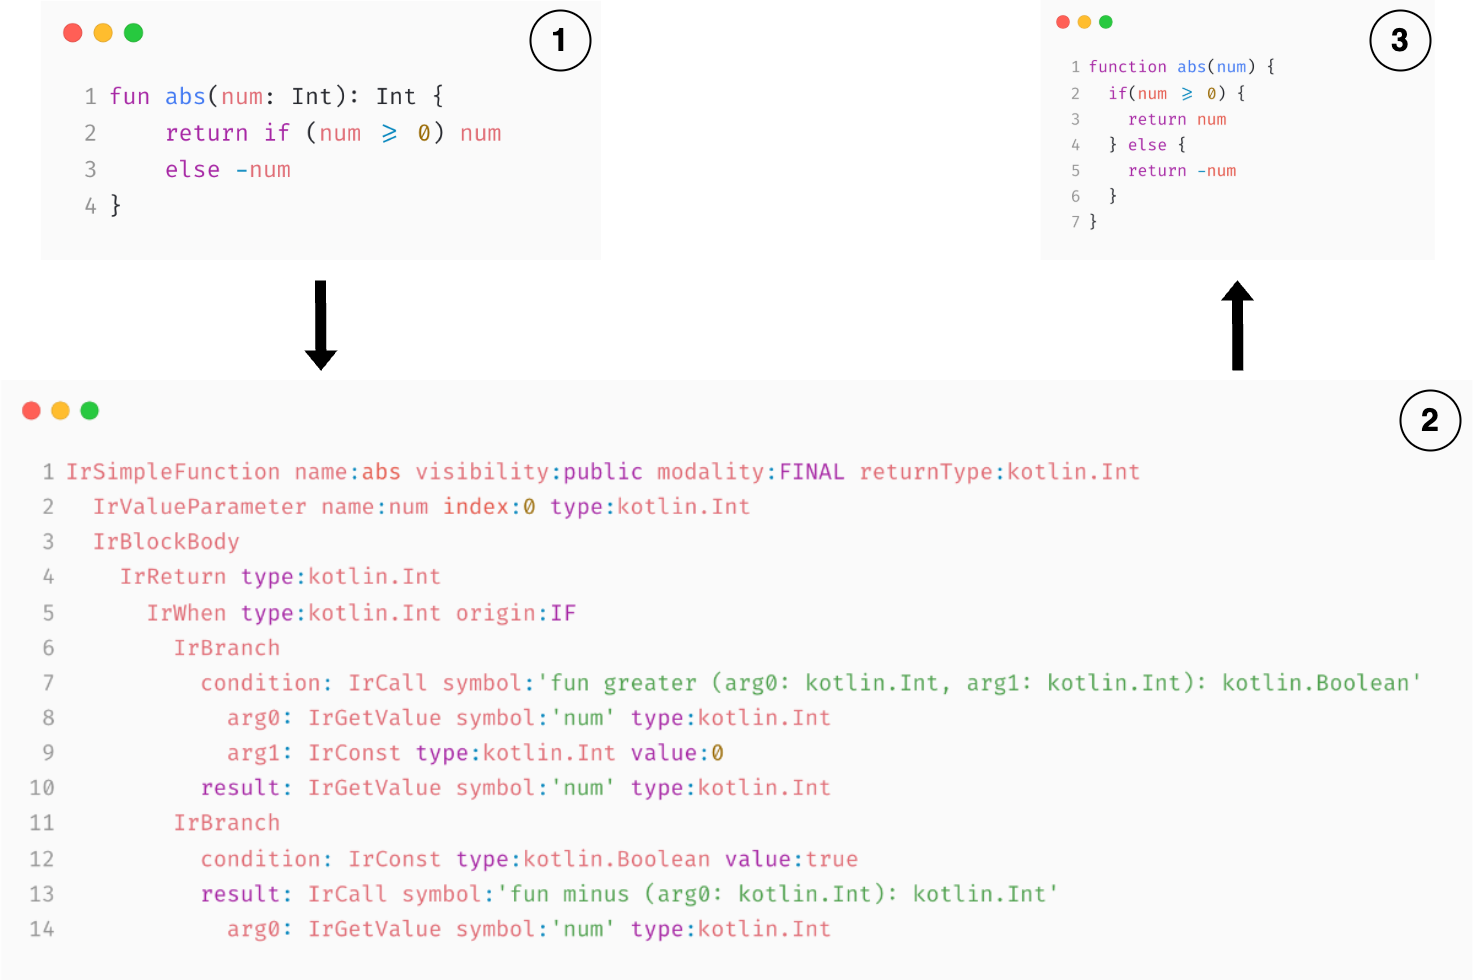
\includegraphics[width=1\textwidth]{charts/kotlin-js-ir.drawio.png}
    \caption{Proces transformacji kodu Kotlin do kodu JavaScript [źródło:~opracowanie~własne na bazie repozytorium kompilatora IR \cite{kotlinIrCompilatorGithub}]}
    \label{fig:kotlin_js_ir}
\end{figure}

Istotnym elementem Kotlin/JS jest wsparcie dla dwóch środowisk wykonawczych: Node.js oraz przeglądarkowego.
W przypadku przeglądarek Kotlin oferuje wsparcie dla DOM API (ang. Document Object Model) \cite{kotlinlangKotlinDocs}, co pozwala na łatwiejszy rozwój aplikacji klienckich działających w przeglądarce.
Ważniejsze dla AWS Lambda jest jednak wsparcie dla Node.js, który jest środowiskiem wykonawczym wspieranym przez usługę.
Wybór środowiska jest łatwo określany poprzez konfigurację narzędzia budującego (np. Gradle) \cite{kotlinlangKotlinDocs}.

Język JavaScript jest znacznie wspierany przez liczną społeczność programistów, co skutkuje bardzo szeroką ofertą różnych bibliotek i frameworków.
Dlatego kluczowym elementem narzędzi jak Kotlin/JS jest wsparcie dla tych aspektów języka.
Po pierwsze, Kotlin/JS pozwala na bezpośrednie użycie kodu JavaScript z Kotlina, poprzez użycie funkcji ,,js()'' \cite{kotlinlangKotlinDocs}.
Z jej użyciem programista może przekazać dowolny kod JavaScript, który zostanie wykonany w miejscu użycia funkcji.
Co więcej, Kotlin Multiplatform oferuje możliwość użycia bibliotek z menadżera pakietów NPM.
Wymaga to od programisty deklaracji tej zależności w konfiguracji Gradle, która jest podobna do deklaracji zwykłych zależności.
Po tym, może on użyć specjalnej annotacji ,,JsModule'' wraz z słowem kluczowym ,,external'', które pełnią rolę adaptera \cite{kotlinlangKotlinDocs}.
Wynika to z dynamicznego typowania JavaScript oraz stytycznego Kotlina. 
Dla zapewnienia lepszych doświadczeń programisty, Kotlin/JS umożliwia także wygenerowanie typów TypeScript \cite{kotlinlangKotlinDocs}.
Mogą być one użyte w przypadu np. udostępnienia biblioteki napisanej z użyciem Kotlin/JS.
Samo zapewnienie integracji z zewnętrznymi bibliotekami jest kluczowe w przypadku AWS Lambda, które wymaga integracji z np. AWS SDK.

Kolejnym ważnym aspektem AWS Lambda jest zmniejszanie wielkości artefaktu \cite{8116416}\cite{9095731}.
W przypadku Kotlin/JS oferowane jest kilka mechanizmów, które mogą pozytywnie wpłynąć na jego rozmiar.
Między innymi zapewnia on narzędzie DCE (ang. dead code elimination), które jest wbudowane w kompilator IR.
Polega ono na eliminacji kodu, który nie jest wykorzystywany w aplikacji.
Mogą to być na przykład funkcje z biblioteki standardowej Kotlina, które nie zostały użyte w kodzie funkcji.
Dodatkowo, aby kod Kotlin został przekonwertowany do kodu JavaScript, musi zostać użyta annotacja ,,@JsExport'' \cite{kotlinlangKotlinDocs}.
Dzięki temu, oznaczone nią funkcje czy klasy są traktowane jako elementy źródłowe dla mechanizmu DCE, co rozpocznie analizę używanego kodu właśnie od nich.
Dodatkowo, kompilator dokonuje minifikacji (ang. minification) nazw, jak zmienne.
Wszystko to pozwala na osiągnięcie mniejszego rozmiaru artefaktu, co jest istotnym aspektem w optymalizacji wydajności AWS Lambda.

Kotlin/JS posiada jednak także ograniczenia, które mogą negatywnie wpłynąć na rozwój oprogramowania.
Po pierwsze, mimo integracji z bibliotekami zewnętrznymi, może wymagać ona znacznych nakładów pracy.
Wynika to z użycia słowa kluczowego ,,external'' i potrzeby utrzymywania kodu, który zawiera typy bibliotek zewnętrznych.
Może to znacząco spowolnić wszelkie zmiany wersji bibliotek, które mogą zmienić swoje interfejsy.
Dodatkowo, Kotlin/JS posiada znaczne ograniczenia w mechanizmie refleksji.
Nie implementuje on całego API reflekcji Kotlina, a jednymie referencję klasy (::class), typy KType i KClass oraz powiązane z nimi funkcje ,,typeof()'' (zwracającą typ) i ,,createInstance()'' (tworzącą nową instancję klasy).
Czynniki te powinny być uwzględnione w przypadku wyboru Kotlin/JS jako technologii systemu działającego w AWS Lambda.

% 0. Wstęp

% 1. Sposób działania:
% Kotlin\JS jako docelowa platforma. Kod kotlin -> JavaScript
% Jak to działa? - Kompilator IR
% Wsparcie dla browser lub node.js

% 2. Integracja z JS:
% Wsparcie dla bibliotek i kodu JS z Kotlina
% Generowanie typów typescript

% 3. Wielkość artefaktu (ważne w AWS Lambda):
% Wsparcie dla webpacka (czy dla node.js też?)
% Dead Code Elimination i @JsExport
% Minification - jak to przetłumaczyć?

% 4. Ograniczenia:
% Reflection jako ograniczenie

% Linki:
% https://kotlinlang.org/docs/js-overview.html
% https://kotlinlang.org/docs/js-ir-compiler.html
% https://kotlinlang.org/docs/javascript-dce.html
% https://kotlinlang.org/docs/js-ir-compiler.html#minification-of-member-names-in-production
% https://kotlinlang.org/docs/js-ir-compiler.html#current-limitations-of-the-ir-compiler - końcówka, zawrzeć odnośnie JsExport
% https://kotlinlang.org/docs/js-ir-compiler.html#preview-generation-of-typescript-declaration-files-d-ts - typescript
% https://kotlinlang.org/docs/dynamic-type.html - do używania kodu JS z Kotlina
% https://kotlinlang.org/docs/using-packages-from-npm.html - używanie NPM
% https://kotlinlang.org/docs/js-to-kotlin-interop.html#kotlin-types-in-javascript - używanie kotlina z JS (?)
% https://kotlinlang.org/docs/js-reflection.html - reflection jako ograniczenie